\begin{center}
\section{\Large Deduza $A$ o Determinante 4x4 usando a fórmula de Leibniz}
\end{center}


O calculo da determinante da matriz poderá ser feito sem a necessidade de realizar eliminações ou outros métodos complexos, para isso o iremos utilizar o método de Leibniz. Esse processo nos permite a obtenção do valor exato do determinante.

\onehalfspacing
Pode-se considerar a Matriz $A$ como:

\[
A = \begin{bmatrix}
a_{11} & a_{12} & a_{13} & a_{14} \\
a_{21} & a_{22} & a_{23} & a_{24} \\
a_{31} & a_{32} & a_{33} & a_{34} \\
a_{41} & a_{42} & a_{43} & a_{44} \\
\end{bmatrix}
\]

\onehalfspacing
\begin{center}
O determinante de $A$ usando a fórmula de Leibniz é dado por:
\end{center}

\[
\det(A) = \sum_{\sigma \in S_4} (\operatorname{sgn}(\sigma)) \cdot a_{1,\sigma_1} \cdot a_{2,\sigma_2} \cdot a_{3,\sigma_3} \cdot a_{4,\sigma_4}
\]

Onde $\sigma$ percorre todas as permutações possíveis dos índices de 1 a 4, $S_4$ é o conjunto de todas as permutações de 4 elementos, $\operatorname{sgn}(\sigma)$ é o sinal da permutação $\sigma$, e $a_{i,\sigma_i}$ representa o elemento da matriz $A$ na linha $i$ e coluna $\sigma_i$.

\vspace{1cm}

O determinante de A usando a fórmula de Leibniz é dado por:

\begin{center}
$det(A) = (+1) * a11 * a22 * a33 * a44
- a11 * a22 * a34 * a43
+ a11 * a23 * a34 * a42
- a11 * a23 * a32 * a44
+ a11 * a24 * a32 * a43
- a11 * a24 * a33 * a42
- a12 * a21 * a33 * a44
+ a12 * a21 * a34 * a43
- a12 * a23 * a34 * a41
+ a12 * a23 * a31 * a44
- a12 * a24 * a31 * a43
+ a12 * a24 * a33 * a41
+ a13 * a21 * a32 * a44
- a13 * a21 * a34 * a42
+ a13 * a22 * a34 * a41
- a13 * a22 * a31 * a44
+ a13 * a24 * a31 * a42
- a13 * a24 * a32 * a41
- a14 * a21 * a32 * a43
+ a14 * a21 * a33 * a42$
\end{center}

\newpage

\begin{center}
\section{\Large Calcule o Determinante usando o que foi deduzido de duas matrizes definidas pelo autor}
\end{center}

\hspace{1.5cm}
Determinante da primeira Matriz:

\[
A = \begin{bmatrix}
1 & 2 & 3 & 4 \\
2 & 4 & 6 & 8 \\
3 & 6 & 9 & 12 \\
4 & 8 & 12 & 16 \\
\end{bmatrix}
\]

Possui o seguinte determinante:

\begin{Large}  
\[
\det(m) = 0
\]
\end{Large}

\vspace{1cm}

\hspace{1.5cm}
Determinante da primeira Matriz:

\[
A = \begin{bmatrix}
1 & 2 & 3 & 4 \\
0 & 2 & 3 & 4 \\
0 & 0 & 3 & 4 \\
0 & 0 & 0 & 4 \\
\end{bmatrix}
\]

Possui o seguinte determinante:

\begin{Large}  
\[
\det(m) = 24
\]
\end{Large}

\newpage

\begin{center}
\section{\Large Metódo em Python}
\end{center}

\begin{figure}[!htpb]
    \centering
    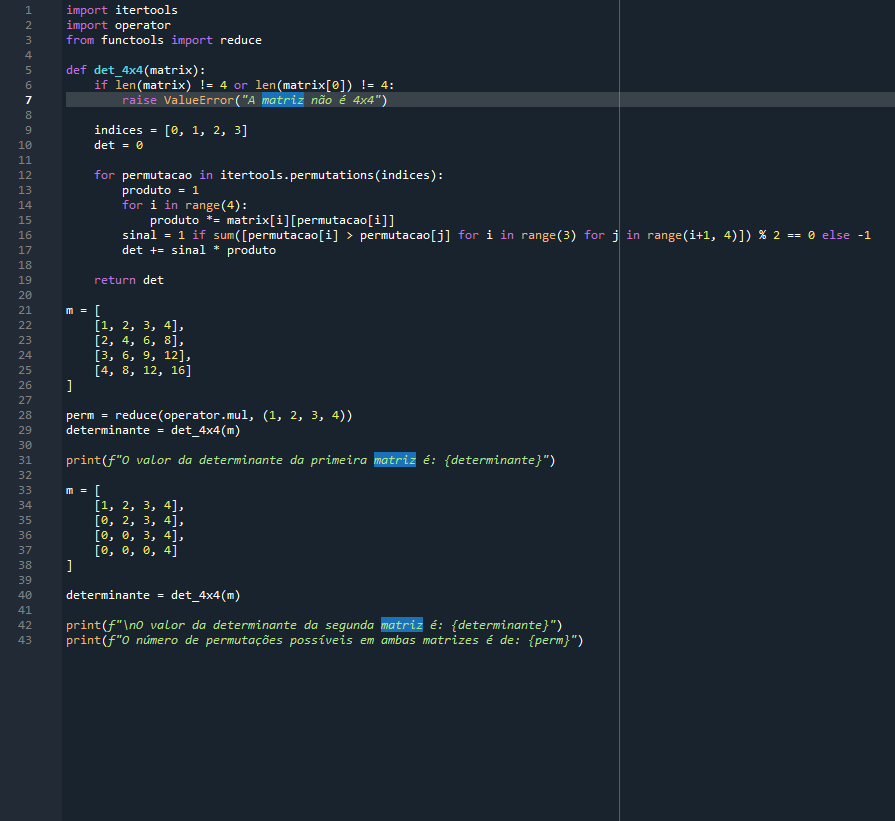
\includegraphics[width=170mm]{code.png}
\end{figure}

\newpage

\begin{center}
\section{\Large Desenvolvimento em Python}
\end{center}

O código implementa a função $det_4x4(matrix)$ em Python para calcular o determinante de matrizes 4x4 usando a Lei de Leibniz.A função gera todas as permutações possíveis dos índices das colunas da matriz, calcula o produto dos elementos correspondentes em cada permutação e acumula o resultado final, levando em conta o sinal apropriado para cada permutação. 

Ao final o código imprime na tela os determinantes de duas matrizes 4x4 predefinidas, juntamente com o número de permutações possíveis.

\vspace{1cm}

\begin{figure}[!htpb]
    \centering
    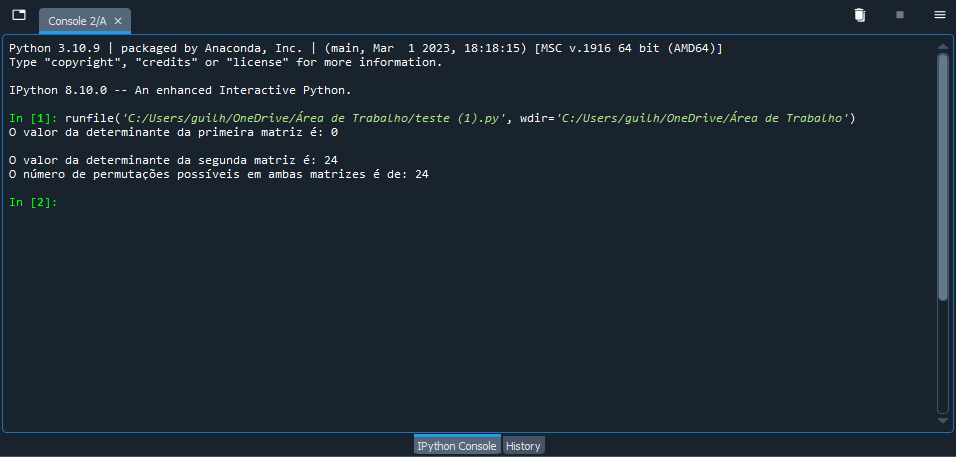
\includegraphics[width=170mm]{console.png}
\end{figure}
